\chapter{Sistema de Ingresso e Versionamento}
\label{chap:historicoversoes}

Neste capítulo são descritas as informações sobre as funcionalidades desenvolvidas no sistema de ingresso do \gls{IFSC} com relação aos requisitos e algoritmos do sistema de cotas. Para esse fim, foi utilizado o histórico do controle de versão no que concerne ao quantitativo de arquivos, classes, funções/métodos e as diferentes versões desde o surgimento da demanda de cotas na legislação.

\section{Histórico de Projeto}
\label{historicopj}
Criado em meados do ano de 2000, o sistema de ingresso do \gls{IFSC}, tem por objetivo disponibilizar vagas de cursos para os discentes do \gls{IFSC}. Esse sistema foi desenvolvido internamente na linguagem PHP, para automatizar os processos seletivos que eram realizados por meio de planilhas e ferramentas não integradas, as quais demandavam ao setor responsável muitas pessoas e muitos procedimentos operacionais repetitivos, gerando falhas no processo por erro humano.

O projeto não utiliza conceitos de orientação a objetos, em sua maioria os arquivos PHP ultrapassam duas mil linhas, sem divisão em camadas \gls{MVC}, com combinações das linguagens Javascript, HTML e PHP no mesmo arquivo. Quando era preciso criar ou adaptar alguma nova funcionalidade por falta de conhecimento técnico, os antigos desenvolvedores (bolsistas) faziam a cópia das funcionalidades para vários locais do sistema, sem pensar em reutilização de código.

Com objetivo de elencar a situação atual do código fonte do sistema, neste trabalho são apresentados os quantitativos levantados a partir do sistema de controle de versão do \gls{IFSC}. A Tabela \ref{quadro_git_ingresso} apresenta o levantamento geral sobre o total de arquivos, linhas de código, commits e desenvolvedores que já atuaram no projeto. Nas Seções seguintes são contextualizados os dados gerais sobre o algoritmo de classificação, assim como é descrito o levantamento feito nas 3 (três) versões do algoritmo de classificação que foram implementadas até o momento.

\begin{quadro}
\caption{Dados gerais do controle de versão}
\label{quadro_git_ingresso}
\centering
\begin{tabular}{ l l }
   \cline{1-1}\cline{2-2}  
    \multicolumn{1}{|p{5.850cm}|}{\textbf{Total de arquivos}} &
    \multicolumn{1}{p{8.217cm}|}{1.357 arquivos (php, html, css, js )}
  \\ 
   \cline{1-1}\cline{2-2}  
    \multicolumn{1}{|p{5.850cm}|}{\textbf{Total de linhas de código}} &
    \multicolumn{1}{p{8.217cm}|}{36.9414 linhas}
  \\    
   \cline{1-1}\cline{2-2}  
    \multicolumn{1}{|p{5.850cm}|}{\textbf{Total de commits}} &
    \multicolumn{1}{p{8.217cm}|}{731}
  \\    
   \cline{1-1}\cline{2-2}  
    \multicolumn{1}{|p{5.850cm}|}{\textbf{Total de desenvolvedores}} &
    \multicolumn{1}{p{8.217cm}|}{6}
  \\     
   \cline{1-1}\cline{2-2}  
    \multicolumn{1}{|p{5.850cm}|}{\textbf{Período da coleta}} &
    \multicolumn{1}{p{8.217cm}|}{11/02/2015 - 17/04/2019}
  \\       
  \hline

 \end{tabular} 
\end{quadro}


\section{Algoritmo de Classificação}
\label{algoritimodeclassificacao}

Nesta Seção são detalhados os conceitos e as etapas do processo de classificação de candidatos às vagas do sistema de cotas, assim como o levantamento de cenários ilustrativos sobre a distribuição de vagas tendo como base as versões já implementadas no sistema de ingresso.

Para cada processo seletivo há uma lista de cursos, em que o setor que gerencia as vagas define-as com base no valor total inicial e indica se o processo seletivo vai utilizar a regra de classificação por cotas. Durante as inscrições são apresentados aos candidatos os campos necessários para indicar se vieram de escola pública, bem como informar a sua renda familiar e se autodeclararem pretos, pardos ou indígenas.

Após o término do período de inscrições, os candidatos são separados em categorias de concorrência de acordo com o preenchimento realizado no ato da inscrição. A seguir, os candidatos participam do processo seletivo de forma física como provas de vestibular ou processos eletrônicos de classificação, como por exemplo: sorteio, pontuação por preenchimento de formulários sócio-econômicos ou classificação por \gls{ENEM} ou \gls{SISU}. Por fim é gerado um número de classificação que representa a ordem dos candidatos que disputam as vagas disponíveis.

O algoritmo de classificação utiliza como parâmetro de entrada a lista de candidatos, contendo o número de inscrição, a ordem de classificação geral, a data de nascimento (como critério de desempate), a quantidade de vagas total do curso, o percentual de vagas disponíveis para escola pública e o percentual de proporção do \gls{IBGE}.

Esses parâmetros variam conforme a Unidade Federada e é fornecido pelo último censo demográfico, representando o percentual sobre o total de pretos, pardos e indígenas no estado em relação às demais categorias de cotas para estudantes da escola pública.

Com esses parâmetros de entrada, o algoritmo gera um quadro de vagas contendo quantas vagas estão reservadas para às respectivas categorias de cotas, e faz a seleção e aprovação de candidatos de acordo com a sua classificação e critérios de desempate. Por fim, em caso de sobra de vagas por falta de candidatos para uma determinada categoria de cota, o algoritmo faz nova busca por candidatos de outra categoria, de acordo com a ordem de prioridade estabelecida na portaria Nº 18 de 2012 do \gls{MEC}, a qual define:

\begin{citacao}
Art. 15. No caso de não preenchimento das vagas reservadas aos autodeclarados pretos, pardos
e indígenas e às pessoas com deficiência, aquelas remanescentes serão preenchidas pelos
estudantes que tenham cursado integralmente o ensino fundamental ou médio, conforme o caso,
em escolas públicas, observadas as reservas realizadas em mesmo nível ou no imediatamente
anterior, nos termos do art. 10 desta Portaria. \cite{portarianr9}
\end{citacao}

No fim do processo de classificação é gerada uma lista de candidatos aprovados, incluindo a classificação geral e a classificação na respectiva categoria de cota, por fim esta lista é enviada ao sistema acadêmico para que os candidatos possam realizar a matrícula e entregar a documentação necessária. 

As alterações nos documentos de lei podem incluir novas categorias, novas formas de distribuição das vagas iniciais, mudanças de percentuais, formas de arredondamento, descrição dos tipos de cotas e mudança na ordem de prioridade em caso de sobra de vagas. Essas situações são exemplificadas nas Seções seguintes por meio dos casos e cenários nos quais houve maior impacto de refatoração de código do sistema de ingresso para adequação à legislação.

\subsection{Versão 1 - Início do sistema de Cotas, Lei Nº 12.711 de 2012}
\label{versao1}

Inicialmente o sistema de ingresso foi construído sem considerar cotas, ou seja, a classificação era por pontuação ou nota de vestibular, não havia exigência de lei em função de reserva de vagas. As chamadas para matrículas eram realizadas pela ordem geral de classificação e alguns critérios de desempate. Hoje apenas alguns tipos de processos seguem este molde, como por exemplo cursos de curta duração, ou cursos internos que não se aplicam à legislação.

Com o surgimento da lei Nº 12.711/2012 vem também a demanda do governo para que as instituições reservem 50\% das vagas para estudantes do ensino médio exclusivamente em escolas públicas, e dentro destes 50\% deveria ser reservado um percentual para estudantes cuja renda familiar fosse inferior a 1.5 salários mínimos per capita:

\begin{citacao}
Parágrafo único.  No preenchimento das vagas de que trata o caput deste artigo, 50\% (cinquenta por cento) deverão ser reservados aos estudantes oriundos de famílias com renda igual ou inferior a 1,5 salário-mínimo (um salário-mínimo e meio) per capita.

Art. 3o  Em cada instituição federal de ensino superior, as vagas de que trata o art. 1o desta Lei serão preenchidas, por curso e turno, por autodeclarados pretos, pardos e indígenas, em proporção no mínimo igual à de pretos, pardos e indígenas na população da unidade da Federação onde está instalada a instituição, segundo o último censo do Instituto Brasileiro de Geografia e Estatística (IBGE) \cite{leicotas}.
\end{citacao}

Com este objetivo o algoritmo de classificação que era uma consulta SQL foi separado em 3 funções PHP de nome: \textit{calcula\_vagasAcoesAfirmativas}, \textit{aprova\_Candidatos} e \textit{retorna\_OrdemdePreenchimentodeVagasNaoOcupadas}.  A primeira com função de gerar o quadro de vagas, a segunda a seleção dos candidatos para serem aprovados e atualizar a contagem de vagas em cada categoria e a ultima para retornar a ordem de preenchimento em caso de sobra de vagas.

Tendo em vista que há uma divisão categórica das vagas entre os candidatos, foi preciso criar 5 (cinco) tipos de situações de classificação para cada combinação de cotas possível, essas categorias foram definidas conforme o Quadro \ref{tabela_categoriasv1}.

\begin{quadro}
\caption{Lista de categorias de cotas da versão 1}
\label{quadro_categoriasv1}
\centering
\begin{tabular}{ l l }
   \cline{1-1}\cline{2-2}  
    \multicolumn{1}{|p{5.850cm}|}{\textbf{CLAG}} &
    \multicolumn{1}{p{8.217cm}|}{Ampla concorrência ou classificação geral 
( todos os candidatos concorrem )}
  \\ 
   \cline{1-1}\cline{2-2}  
    \multicolumn{1}{|p{5.850cm}|}{\textbf{EPRIPPI}} &
    \multicolumn{1}{p{8.217cm}|}{Candidatos que estudaram em Escola Pública com Renda Inferior a 1.5 salários mínimos per capita e autodeclarados Pretos, Pardos ou Indígenas}
  \\    
   \cline{1-1}\cline{2-2}  
    \multicolumn{1}{|p{5.850cm}|}{\textbf{EPRINPPI}} &
    \multicolumn{1}{p{8.217cm}|}{Candidatos que estudaram em Escola Pública com Renda Inferior a 1.5 salários mínimos per capita NÃO são autodeclarados Pretos, Pardos ou Indígenas; }
  \\    
   \cline{1-1}\cline{2-2}  
    \multicolumn{1}{|p{5.850cm}|}{\textbf{EPRSPPI}} &
    \multicolumn{1}{p{8.217cm}|}{Candidatos que estudaram em Escola Pública com Renda Superior a 1.5 salários mínimos per capita e autodeclarados Pretos, Pardos ou Indígenas}
  \\     
   \cline{1-1}\cline{2-2}  
    \multicolumn{1}{|p{5.850cm}|}{\textbf{EPRSNPPI}} &
    \multicolumn{1}{p{8.217cm}|}{Candidatos que estudaram em Escola Pública com Renda Superior a 1.5 salários mínimos per capita NÃO são autodeclarados Pretos, Pardos ou Indígenas}
  \\       
  \hline

 \end{tabular} 
\end{quadro}


\newpage
Dadas as situações de classificação possíveis o primeiro passo do algoritmo é gerar um quadro de vagas para cada tipo de cota, tendo como base o percentual do \gls{IBGE} e o total de vagas para o curso. O trecho de código desenvolvido será apresentado no Código Fonte \ref{lst:quadrovagas}.


\lstinputlisting[language=PHP, 
caption=Função que calcula o quadro de vagas
,label=lst:quadrovagas]{chapters/trechos_codigo/calculaquadrovagas.m}

Basicamente o que a função \textit{calcula\_vagasAcoesAfirmativas} faz é separar as vagas o seguinte passo a passo:

\begin{enumerate}
    \item Dado o total de vagas do curso;
    \item Obter o percentual de escola pública;
    \item Obter o percentual de proporção de PPI do IBGE no estado de oferta;
    \item Multiplicar o total de vagas pelo percentual de Escola Pública (50\%) e armazenar o valor em AAEP;
    \item Obter o total reservado para ampla concorrência (CLAG), diminuindo o total de vagas pelo reservado ao sistema de cotas AAEP;
    \item Dividir o total de vagas AAEP em 50\% para candidatos de Renda Inferior a 1.5 (AAEPRI) e 50\% para candidatos de Renda Superior a 1.5 (AAEPRS);
    \item Dentro do total de vagas AAEPRI, deve-se calcular a proporção reservada pelo IBGE para cotistas PPI (Preto, Pardo, Indígenas) que também possuam Renda Inferior a 1.5 salários mínimos e armazenar em AAEPRIPPI;
    \item O total de vagas de estudantes de Renda Inferior que NÃO são autodeclarados PPI (AAEPRINPPI) é obtido após diminuir o total de vagas para renda inferior AAEPRI - o total armazenado em (AAEPRIPPI).
    \item Dentro do total de vagas AAEPRS, deve-se calcular a proporção reservada pelo IBGE para cotistas PPI (Preto, Pardo, Indígenas) que também possuam Renda Superior a 1.5 salários mínimos e armazenar em AAEPRSPPI;
    \item O total de vagas de estudantes de Renda Superior que NÃO são autodeclarados PPI (AAEPRSNPPI) é obtido após diminuir o total de vagas para renda inferior AAEPSI - o total armazenado em (AAEPRSPPI).
\end{enumerate}{}

Um exemplo do resultado da geração do quadro de vagas, para um cenário de curso com 40 vagas,  pode ser visto na Figura \ref{fig:cenario1}.

\begin{figure}[ht!]
\centering

\caption{\textmd{Cenário de distribuição versão 1}}
\label{fig:cenario1}
\fcolorbox{gray}{white}{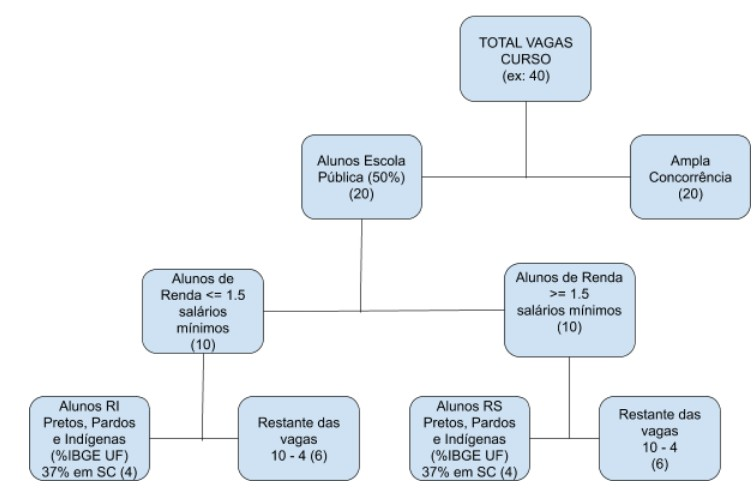
\includegraphics[width=0.67\textwidth]{chapters/sistemaingresso_versoes/cenarios/cenario1.jpg}}

\par\medskip\textbf{Fonte:} Elaborada pelo autor (2019). \par\medskip
\end{figure}



\newpage
Tendo com base o quadro de vagas o algoritmo de classificação de candidatos utiliza a função \textit{aprova\_Candidatos} descrita no Código Fonte \ref{lst:algoritmoaprovacao}, fazendo a seleção dos candidatos para aprovação em cada categoria até atingir o total de vagas disponível. 

\lstinputlisting[language=PHP, 
caption=Função de aprovação de candidatos
,label=lst:algoritmoaprovacao]{chapters/trechos_codigo/aprovacandidatos.m}

Por fim, o algoritmo utiliza a função \textit{retorna\_OrdemdePreenchimentodeVagasNaoOcupadas} obter a prioridade por lei quando sobra vaga de uma determinada categoria de cota, por motivo de falta de candidatos inscritos (Código Fonte \ref{lst:sobravagas}).

\lstinputlisting[language=PHP, 
caption=Função de prioridade em caso de sobra de vagas
,label=lst:sobravagas]{chapters/trechos_codigo/sobravagas.m}

Após análise no controle de versão pode-se identificar que as funções eram utilizadas em diferentes etapas e tipos de processo do sistema. No entanto a equipe que desenvolveu o sistema não teve preocupação na organização do código e fez a cópia em vários pontos do sistema, trazendo ainda mais problemas de manutenção no sistema. Os arquivos envolvidos, assim como os dados do controle de versão serão listados nas Tabelas \ref{tabela_arquivosv1_1}, \ref{tabela_arquivosv1_2}, \ref{tabela_arquivosv1_3} e \ref{tabela_arquivosv1_4}.

\begin{table}[ht!]
\centering
\caption{Versionamento do arquivo corrigir.php}
\label{tabela_arquivosv1_1}
\resizebox{\textwidth}{!}{
\begin{tabular}{@{}|l|l|@{}}
\toprule
\multicolumn{2}{|c|}{ingresso/admin/admin/correcao/corrigir.php}                                        \\ \midrule
\textbf{Total de linhas de código}                               & 1129                                 \\ \midrule
\textbf{Total de funções utilizadas}                             & 267 funções (incluídas e importadas) \\ \midrule
\textbf{Total de funções / algoritmo de cotas}                   & 5 funções                            \\ \midrule
\textbf{Número de linhas envolvidas / algoritmo de cotas}        &                                      \begin{tabular}{@{}|l|l|@{}}
\toprule
\textbf{processar\_Correcao}                             & 96 linhas de código \\ \midrule
\textbf{calcula\_vagasAcoesAfirmativas}                  & 33 linhas de código \\ \midrule
\textbf{aprova\_Candidatos}                              & 73 linhas de código \\ \midrule
\textbf{retorna\_OrdemdePreenchimentodeVagasNaoOcupadas} & 27 linhas de código \\ \midrule
\textbf{alimenta\_Classificacao}                         & 35 linhas de código \\ \bottomrule
\end{tabular}
    \\ \midrule
\textbf{Commits relevantes}                         & 31 commits desde  11/02/2015         \\ \midrule
\textbf{Número de programadores envolvidos nos commits}          & 2                                    \\ \midrule
\textbf{Total de linhas de código para a implementação de cotas} & 264 linhas                           \\ \bottomrule

\end{tabular}}

\par\medskip\textbf{Fonte:} Elaborada pelo autor (2019). \par\medskip

\end{table}

\begin{table}[ht!]
\centering
\caption{Versionamento do arquivo informar\_classificacao01\_sorteio.php}
\label{tabela_arquivosv1_2}
\resizebox{\textwidth}{!}{
\begin{tabular}{@{}|l|l|@{}}
\toprule
\multicolumn{2}{|c|}{ingresso/admin/admin/semprova/informar\_classificacao01\_sorteio.php}                                        \\ \midrule
\textbf{Total de linhas de código}                               & 1360                                 \\ \midrule
\textbf{Total de funções utilizadas}                             & 236 funções (incluídas e importadas) \\ \midrule
\textbf{Total de funções / algoritmo de cotas}                   & 5 funções                            \\ \midrule
\textbf{Commits relevantes}                         & 61 commits desde  11/02/2015         \\ \midrule
\textbf{Número de programadores envolvidos nos commits}          & 2                                    \\ \bottomrule
\end{tabular}}

\par\medskip\textbf{Fonte:} Elaborada pelo autor (2019). \par\medskip
\end{table}

\begin{table}[ht!]
\centering
\caption{Versionamento do arquivo informar\_classificacao01.php}
\label{tabela_arquivosv1_3}
\resizebox{\textwidth}{!}{
\begin{tabular}{@{}|l|l|@{}}
\toprule
\multicolumn{2}{|c|}{ingresso/admin/admin/semprova/informar\_classificacao01.php}                                        \\ \midrule
\textbf{Total de linhas de código}                               & 1162                                 \\ \midrule
\textbf{Total de funções utilizadas}                             & 88 funções (incluídas e importadas) \\ \midrule
\textbf{Total de funções / algoritmo de cotas}                   & 6 funções                            \\ \midrule
\textbf{Commits relevantes}                         & 14 commits desde  11/02/2015         \\ \midrule
\textbf{Número de programadores envolvidos nos commits}          & 2                                    \\ \bottomrule
\end{tabular}}
\par\medskip\textbf{Fonte:} Elaborada pelo autor (2019). \par\medskip
\end{table}

\begin{table}[ht!]
\centering
\caption{Versionamento do arquivo  semprova/classificacao01\_sorteio.php}
\label{tabela_arquivosv1_4}
\resizebox{\textwidth}{!}{
\begin{tabular}{@{}|l|l|@{}}
\toprule
\multicolumn{2}{|c|}{ingresso/admin/admin/semprova/informar\_classificacao01\_sorteio.php}                                        \\ \midrule
\textbf{Total de linhas de código}                               & 1363                                 \\ \midrule
\textbf{Total de funções utilizadas}                             & 119 funções (incluídas e importadas) \\ \midrule
\textbf{Total de funções / algoritmo de cotas}                   & 6 funções                            \\ \midrule
\textbf{Commits relevantes}                         & 24 commits desde  11/02/2015         \\ \midrule
\textbf{Número de programadores envolvidos nos commits}          & 3                                    \\ \bottomrule
\end{tabular}}
\par\medskip\textbf{Fonte:} Elaborada pelo autor (2019). \par\medskip
\end{table}

\newpage
Com base nesse levantamento pode-se observar uma quantidade considerável de código fonte envolvido para desenvolvimento de regras para classificação de candidatos. Como tentativa de dar celeridade no processo de desenvolvimento de correções e na criação de futuras versões, os problemas de código duplicado foram reduzidos por meio de refatoração nas versões posteriores do algoritmo de classificação. Na Seção \ref{versao2} são apresentados os dados sobre o controle de versão, pós refatoração realizada em função de novas demandas de alteração da legislação.


\subsection{Versão 2 - Alteração para Lei Nº 13.409 de 2016 }
\label{versao2}
 Em função da criação da Lei nº 13.409, que altera a lei original nº 12.711, foi feita uma re-estruturação do código para inclusão de novas categorias de cotas para \gls{PCD}, mantendo as outras categorias já existentes. Os trechos de lei afetados foram:
\begin{citacao}
Art. 3º Em cada instituição federal de ensino superior, as vagas de que trata o art. 1º desta Lei serão preenchidas, por curso e turno, por autodeclarados pretos, pardos e indígenas e por pessoas com deficiência, nos termos da legislação, em proporção ao total de vagas no mínimo igual à proporção respectiva de pretos, pardos, indígenas e pessoas com deficiência na população da unidade da Federação onde está instalada a instituição, segundo o último censo da Fundação Instituto Brasileiro de Geografia e Estatística - IBGE.

Art. 5º Em cada instituição federal de ensino técnico de nível médio, as vagas de que trata o art. 4º desta Lei serão preenchidas, por curso e turno, por autodeclarados pretos, pardos e indígenas e por pessoas com deficiência, nos termos da legislação, em proporção ao total de vagas no mínimo igual à proporção respectiva de pretos, pardos, indígenas e pessoas com deficiência na população da unidade da Federação onde está instalada a instituição, segundo o último censo do IBGE \cite{leicotas2}.
\end{citacao}

A equipe de desenvolvimento original do sistema já não estava mais presente no setor e a falta de experiência nas regras de cotas por parte da equipe atual, acabou por dificultar e atrasar o processo de entendimento do código fonte para aplicação das mudanças no sistema,  demandando também a alocação de mais desenvolvedores para divisão do trabalho de codificação dos novos tipos de cota.

Após a análise dos novos trechos de lei foi especificada uma nova versão do algoritmo de classificação, desenvolvida por meio de interpretação da área demandante e dos analistas de sistemas da \gls{DTIC}, o que gerou uma nova implementação contendo 7 (sete) tipos de categorias de cotas possíveis, conforme Tabela \ref{tabela_cotas_v2}:

\begin{table}[!ht]
\caption{Categorias de cotas na versão 2}
\label{tabela_cotas_v2}
\resizebox{\textwidth}{!}{
\begin{tabular}{|l|l|l|}
\hline
\multirow{6}{*}{\textbf{\begin{tabular}[c]{@{}l@{}}Cotas (EP)\\ mínimo 50\% das vagas\end{tabular}}} & \multirow{3}{*}{\begin{tabular}[c]{@{}l@{}}Renda Inferior do que 1,5 S.M.\\ \\ RI 50\% das cotas   \\ \\
\end{tabular}} & PPI – Pretos Pardos e Índios*           \\ \cline{3-3} 
                                                                                                     &                                                                                                                         & PCD – Pessoas com Deficiência*          \\ \cline{3-3} 
                                                                                                     &                                                                                                                         & NPPID – Não incluídos nos casos acima** \\ \cline{2-3} 
                                                                                                     & \multirow{3}{*}{\begin{tabular}[c]{@{}l@{}}Renda Superior a 1,5 S.M.\\ \\ RS 50\% das cotas  \\ \\ \end{tabular}}       & PPI – Pretos Pardos e Índios*           \\ \cline{3-3} 
                                                                                                     &                                                                                                                         & PCD – Pessoas com Deficiência*          \\ \cline{3-3} 
                                                                                                     &                                                                                                                         & NPPID – Não incluídos nos casos acima** \\ \hline
\multicolumn{3}{|l|}{\textbf{\begin{tabular}[c]{@{}l@{}}Classificação Geral (CLAG)\\ \\ vagas restantes além das cotas\\ \\ máximo 50\% das vagas\end{tabular}}}                                                                                                         \\ \hline
\end{tabular}}
\centering
\par\medskip\textbf{Fonte:} Elaborada pelo autor (2019). \par\medskip
\end{table}

\newpage
O desenvolvimento durou cerca de 3 (três) meses, com 2 (dois) desenvolvedores dedicados, os quais trabalharam em todos os arquivos descritos na primeira versão, assim como as telas envolvidas para atender a este novo entendimento e disponibilizar o Código Fonte \ref{lst:algoritmov2}:

\lstinputlisting[language=PHP, 
caption= Segunda versão do algoritmo
,label=lst:algoritmov2]{chapters/trechos_codigo/algoritmov2.m}

Esse algoritmo substitui o corpo da função \texttt{calcula\_vagasAcoesAfirmativas}, detalhada no Código Fonte \ref{lst:quadrovagas}. Como resultado da geração do quadro de vagas na versão 2, a Figura \ref{fig:cenario2} demonstra o novo cenário para um curso com 40 vagas.

\begin{figure}[ht!]
\centering

\caption{\textmd{Cenário de distribuição versão 2}}
\label{fig:cenario2}
\fcolorbox{gray}{white}{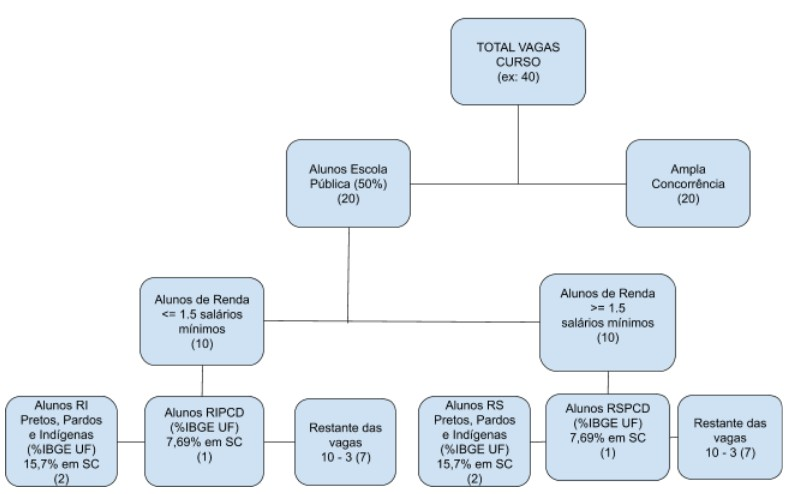
\includegraphics[width=\textwidth]{chapters/sistemaingresso_versoes/cenarios/cenario2.jpg}}

\par\medskip\textbf{Fonte:} Elaborada pelo autor (2019). \par\medskip
\end{figure}



É importante ressaltar que o entendimento de lei repassado pela área demandante se deu sem definição formal do \gls{MEC}, a análise foi procedida por meio de interpretação própria do \gls{IFSC}, e também não havia sido definido como priorizar a sobra de vagas entre cotas, uma vez que a portaria nº 18/2012/MEC  demorou a ser atualizada. Mesmo sem definição clara, o \gls{IFSC} aplicou em seus processos a nova regra de cotas, incluindo a reserva para \gls{PCD}.

Após alguns meses em funcionamento desta versão, o \gls{MEC} em resposta oficial, em função das dúvidas das instituições, acabou por modificar novamente a distribuição de vagas, que agora seria em 9 (nove) categorias de cotas diferentes, e também foram atualizadas as regras de priorização em caso de sobra de vaga. Nesse sentido, na Subseção \ref{versao3} são apresentados os dados de desenvolvimento da versão atualmente utilizada nos processos seletivos.

\subsection{Versão 3 - Reimplementação para interpretação do MEC em 2017 }
\label{versao3}

Com objetivo de unificar o entendimento da distribuição de cotas, o \gls{MEC} lançou em seu portal as alterações e detalhes sobre como deveria ser implementada a nova regra de ingresso em vestibulares e processos seletivos da rede federal. Na Figura \ref{fig:mec} pode-se observar a nova divisão, que agora abrange \gls{PPI} que possuam alguma deficiência e \gls{PPI} que não possuam deficiência, tanto para os estudantes de escolas públicas com renda inferior, como estudantes de renda superior a 1,5 salários mínimos. 

\begin{figure}[ht!]
\centering

\caption{\textmd{Novo procedimento de aplicação do sistema de cotas}}
\label{fig:mec}
\fcolorbox{gray}{white}{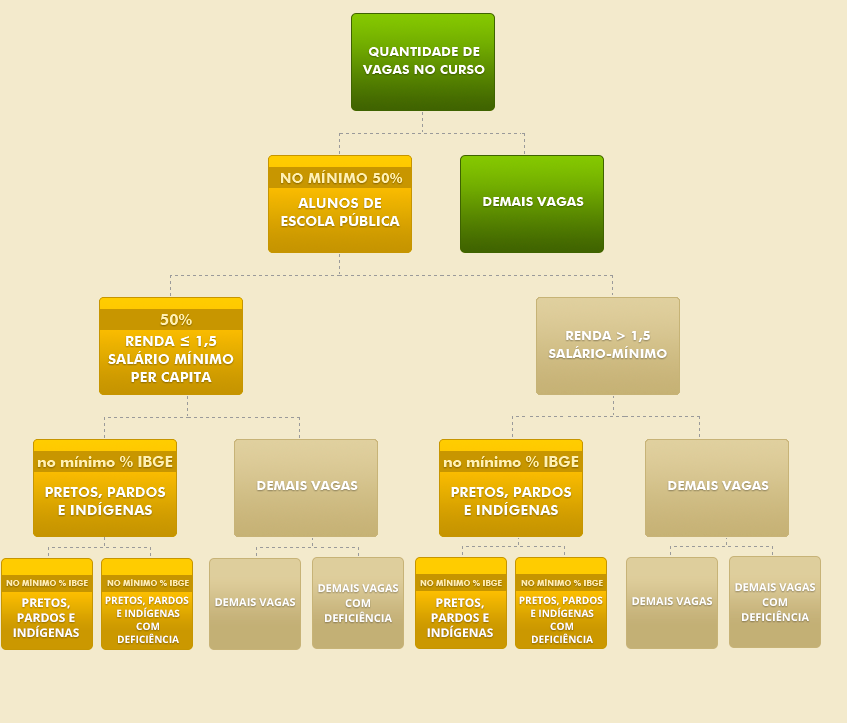
\includegraphics[width=0.67\textwidth]{chapters/sistemaingresso_versoes/imagens/mec.png}}

\par\medskip\textbf{Fonte:} \citeonline{sitemec}. \par\medskip

\end{figure}




Na versão anterior da implementação o aluno teria que optar por concorrer entre uma das opções ou \gls{PPI} ou somente \gls{PCD} ou demais vagas, causando problemas durante as inscrições de várias instituições de ensino, pois haviam candidatos que eram tanto \gls{PPI} como \gls{PCD} e tinham direito a concorrer nas duas categorias de cota.

Tendo em vista a correção do entendimento feita pelo \gls{MEC}, foi preciso criar 9 (nove) tipos de situações de classificação para cada combinação de cotas possível (Tabela \ref{tabela_cotasv3}).

\begin{table}[ht]
\caption{Lista de categorias de cotas da versão 3}
\label{tabela_cotasv3}
\centering
\resizebox{\textwidth}{!}{
\begin{tabular}{ l l }
   \cline{1-1}\cline{2-2}  
    \multicolumn{1}{|p{5.850cm}|}{\textbf{CLAG}} &
    \multicolumn{1}{p{8.217cm}|}{Ampla concorrência ou classificação geral}
  \\ 
   \cline{1-1}\cline{2-2}  
    \multicolumn{1}{|p{5.850cm}|}{\textbf{RIPPIPCDR1}} &
    \multicolumn{1}{p{8.217cm}|}{Renda igual ou inferior a 1,5 (um vírgula cinco) salário-mínimo per capita autodeclarados pretos, pardos ou indígenas com deficiência (PcD PPI).}
  \\    
   \cline{1-1}\cline{2-2}  
    \multicolumn{1}{|p{5.850cm}|}{\textbf{RINPPIPCDR2}} &
    \multicolumn{1}{p{8.217cm}|}{Estudante de escolas públicas brasileiras com renda igual ou inferior a 1,5 (um vírgula cinco) salário-mínimo per capita não autodeclarados pretos, pardos ou indígenas com deficiência (PcD Não PPI)}
  \\
   \cline{1-1}\cline{2-2}  
    \multicolumn{1}{|p{5.850cm}|}{\textbf{RSPPIPCDR3}} &
    \multicolumn{1}{p{8.217cm}|}{
Renda superior a 1,5 (um vírgula cinco) salário-mínimo per capita autodeclarados pretos, pardos, indígenas com deficiência (PcD PPI)}
  \\
  \cline{1-1}\cline{2-2}  
    \multicolumn{1}{|p{5.850cm}|}{\textbf{RSNPPIPCDR4}} &
    \multicolumn{1}{p{8.217cm}|}{
Renda superior a 1,5 (um vírgula cinco) salário-mínimo per capita não autodeclarados pretos, pardos ou indígenas com deficiência (PcD Não PPI)}
  \\
   \cline{1-1}\cline{2-2}  
    \multicolumn{1}{|p{5.850cm}|}{\textbf{RIPPIR5}} &
    \multicolumn{1}{p{8.217cm}|}{
Renda inferior a 1,5 (um vírgula cinco) salário-mínimo per capita autodeclarados pretos, pardos ou indígenas (PPI)}
 \\
   \cline{1-1}\cline{2-2}  
    \multicolumn{1}{|p{5.850cm}|}{\textbf{RINPPIR6}} &
    \multicolumn{1}{p{8.217cm}|}{
Renda inferior a 1,5 (um vírgula cinco) salário-mínimo per capita não autodeclarados pretos, pardos ou indígenas (Não PPI)
}
  \\  
   \cline{1-1}\cline{2-2}  
    \multicolumn{1}{|p{5.850cm}|}{\textbf{RSPPIR7}} &
    \multicolumn{1}{p{8.217cm}|}{
Renda superior a 1,5 (um vírgula cinco) salário-mínimo per capita autodeclarados pretos, pardos ou indígenas (PPI)
}
  \\  
   \cline{1-1}\cline{2-2}  
    \multicolumn{1}{|p{5.850cm}|}{\textbf{RSNPPIR8}} &
    \multicolumn{1}{p{8.217cm}|}{
Renda superior a 1,5 (um vírgula cinco) salário-mínimo per capita não autodeclarados pretos, pardos ou indígenas (Não PPI)
}
  \\   
  \hline

 \end{tabular}}
\end{table}


Tendo como base essas novas categorias, a Figura \ref{fig:cenario3} detalha o terceiro cenário de classificação para um curso de 40 vagas. 

\begin{figure}[ht!]
\centering

\caption{\textmd{Cenário de distribuição versão 3}}
\label{fig:cenario3}
\fcolorbox{gray}{white}{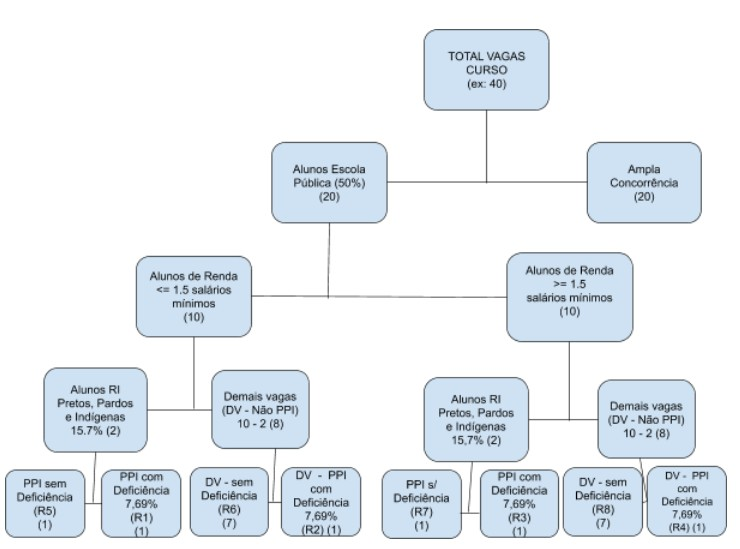
\includegraphics[width=0.9\textwidth]{chapters/sistemaingresso_versoes/cenarios/cenario3.jpg}}

\par\medskip\textbf{Fonte:} Elaborada pelo autor (2019). \par\medskip
\end{figure}



\newpage
Diante da crescente demanda por alterações nas funções de classificação por cotas, a \gls{DTIC} optou por refatorar o código de modo que as regras de distribuição não fossem implementadas de forma estática no código fonte, esta versão foi implementada com armazenamento da árvore de cotas em banco de dados, como uma tentativa de diminuir o impacto em novas mudanças por parte dos desenvolvedores. 

Nesta versão houve uma redução de linhas de código considerável e a equipe centralizou rotinas responsáveis pelos cálculos em apenas um arquivo \textit{calculo\_cotas.php}. As novas funções de cálculo serão descritas nos próximos parágrafos.


\subsection{Outras customizações realizadas no algoritmo}
\label{outrasVersoes}

O \gls{MEC} em sua implementação para classificação de candidatos do \gls{SISU} para o primeiro semestre de 2018, acabou por adotar em seu sistema um entendimento distinto sobre questões de arredondamento de vagas em contra-mão do que era descrito na portaria normativa nº 18/2012/MEC:

\begin{citacao}
Art. 11 - Sempre que a aplicação dos percentuais para a apuração da reserva de vagas de que trata o art. 10 implicar resultados com decimais, será adotado, em cada etapa do cálculo, o número inteiro imediatamente superior \cite{portarianr9}.
\end{citacao}

\begin{figure}[h!]
\centering

\caption{\textmd{Solicitação de correções para processos SISU}}
\label{fig:seres}
\fcolorbox{gray}{white}{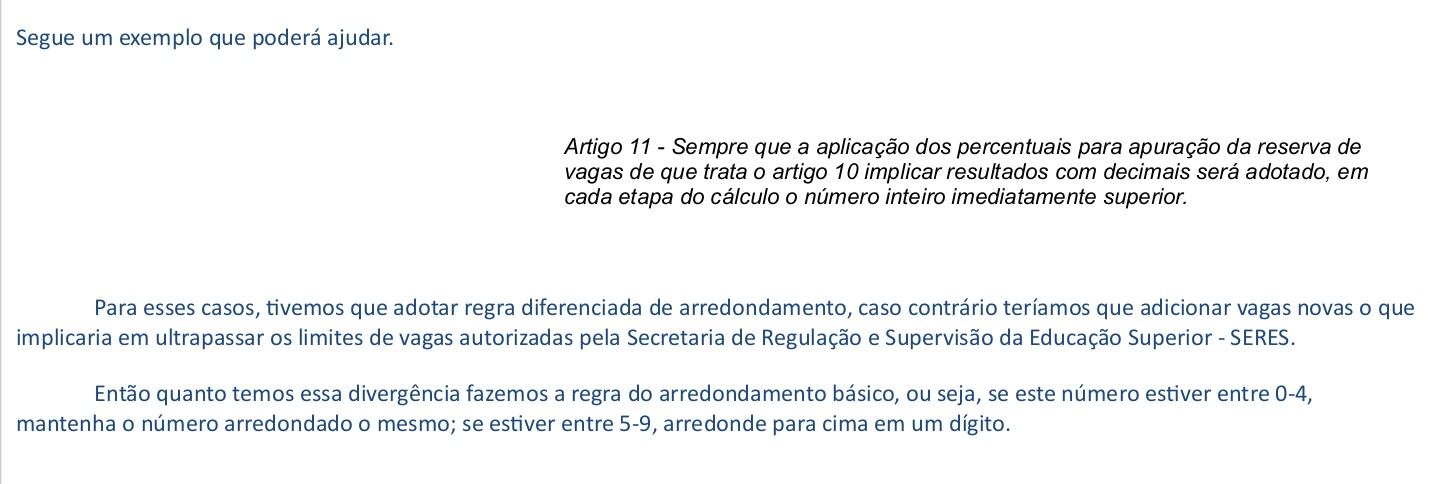
\includegraphics[width=\textwidth]{chapters/sistemaingresso_versoes/imagens/seres.jpg}}

\par\medskip\textbf{Fonte:} Servidor de e-mails do IFSC \par\medskip

\end{figure}



\newpage
A área demandante do \gls{IFSC} em consulta com a \gls{SERES} recebeu o retorno de que tiveram que adotar regra diferenciada de arredondamento do exigido em lei, por questões de limitação de vagas (Figura \ref{fig:seres}), algumas categorias não poderiam ser atendidas na época, obrigando que o sistema de ingresso do \gls{IFSC} fosse ajustado para a modalidade de processos do tipo \gls{SISU}, principalmente para chamada de vagas posteriores à classificação gerada pelo \gls{SISU}.

Nesse contexto, a equipe de desenvolvimento da \gls{DTIC} precisou fazer correções no algoritmo de classificação para considerar o arredondamento diferenciado. Com isso, inseriu novas configurações em banco de dados para o cálculo condicionando à modalidade do processo, mantendo a compatibilidade com processos que seguem a forma de arredondamento prevista em lei.

A exemplo do desenvolvimento necessário para essa correção de arredondamento, o sistema de controle de versão indica como 8 arquivos PHP modificados, sendo 69 linhas adicionadas e 44 linhas removidas, além da necessidade de inclusão de 2 novos campos na tabela de configurações do sistema de cotas (Figura \ref{fig:versaosisu}).

\begin{figure}[h!]
\centering

\caption{\textmd{Controle de versão para correções SISU}}
\label{fig:versaosisu}
\fcolorbox{gray}{white}{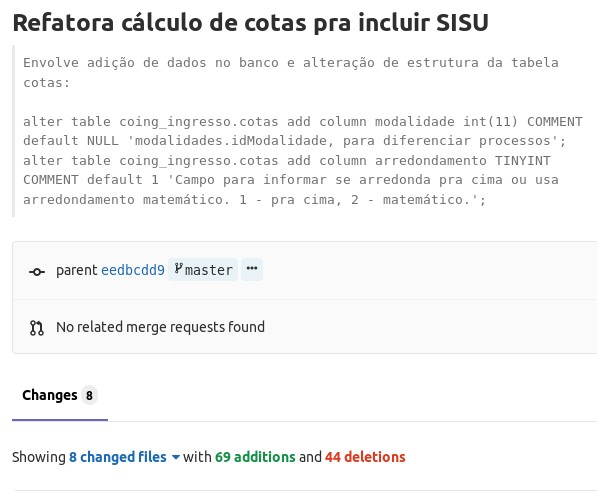
\includegraphics[width=\textwidth]{chapters/sistemaingresso_versoes/imagens/versaosisu.jpg}}

%\par\medskip\textbf{Fonte:} \cite{sitemec} \par\medskip

\end{figure}



\newpage
Essas foram as maiores alterações levantadas no sistema de controle de versões do \gls{IFSC}, no entanto, pode-se observar nas Figuras \ref{fig:chamados} e \ref{fig:trello}, que foram criadas várias demandas na ferramenta \textit{Trello} (utilizada para gerenciamento do desenvolvimento interno), assim como vários chamados de cunho corretivo.  

\begin{figure}[ht!]
\centering

\caption{\textmd{Chamados sobre cotas no sistema de ingresso}}
\label{fig:chamados}
\fcolorbox{gray}{white}{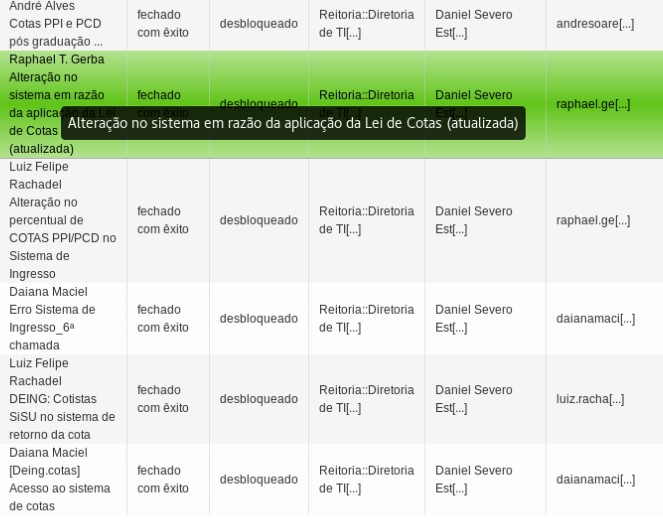
\includegraphics[width=0.7\textwidth]{chapters/sistemaingresso_versoes/imagens/chamados.jpg}}
\par\medskip\textbf{Fonte:} Elaboração do autor \par\medskip

\end{figure}



\begin{figure}[h!]
\centering

\caption{\textmd{Demandas sobre o desenvolvimento de cotas}}
\label{fig:trello}
\fcolorbox{gray}{white}{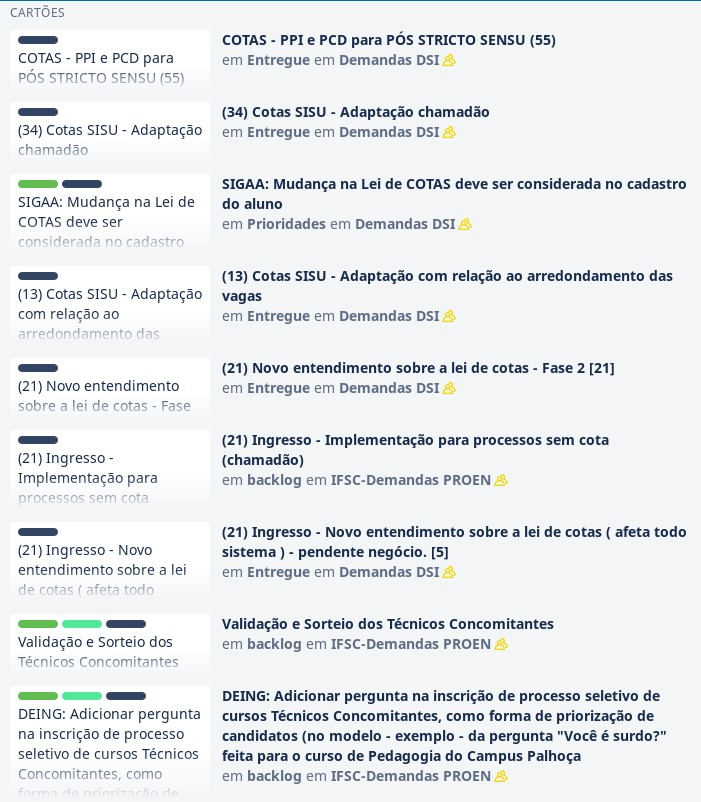
\includegraphics[width=\textwidth]{chapters/sistemaingresso_versoes/imagens/trello.jpg}}

%\par\medskip\textbf{Fonte:} \cite{sitemec} \par\medskip

\end{figure}



\newpage
Tendo em vista os problemas de desenvolvimento ligados ao histórico de versões citados anteriormente, o Capítulo \ref{chap:fundamentacao} aborda conceitos sobre \gls{DSL}, como uma maneira de abstrair questões técnicas de programação para fins de definição e implementação de regras de negócio. Serão elencadas as principais vantagens e desvantagens da \gls{DSL} em relação à \gls{GPL} conforme a literatura, assim como as ferramentas mais utilizadas para construção de linguagens específicas de domínio.





